% author:   sam tenka
% change:   2022-05-24
% create:   2022-05-11

%==============================================================================
%====  0.  DOCUMENT SETTINGS  ================================================
%==============================================================================

%~~~~~~~~~~~~~~~~~~~~~~~~~~~~~~~~~~~~~~~~~~~~~~~~~~~~~~~~~~~~~~~~~~~~~~~~~~~~~~
%~~~~~~~~~~~~~  0.0. About this Exposition  ~~~~~~~~~~~~~~~~~~~~~~~~~~~~~~~~~~~

%---------------------  0.0.0. page geometry  ---------------------------------
\documentclass[11pt, justified]{tufte-book}
\geometry{
  left           = 0.90in, % left margin
  textwidth      = 4.95in, % main text block
  marginparsep   = 0.15in, % gutter between main text block and margin notes
  marginparwidth = 2.30in, % width of margin notes
                 % 0.20in  % width from margin to edge
}

%---------------------  0.0.1. math packages  ---------------------------------
\newcommand\hmmax{0} % to allow for more fonts 
\newcommand\bmmax{0} % to allow for more fonts
\usepackage{amsmath, amssymb, amsthm, mathtools}
\usepackage{bm}
\usepackage{euler}

\usepackage{array}   % for \newcolumntype macro
\newcolumntype{L}{>{$}l<{$}} % math-mode version of "l" column type
\newcolumntype{C}{>{$}c<{$}} % math-mode version of "c" column type
\newcolumntype{R}{>{$}r<{$}} % math-mode version of "r" column type

%---------------------  0.0.2. graphics packages  -----------------------------
\usepackage{graphicx, xcolor}
\usepackage{float, capt-of}

%---------------------  0.0.3. packages for fancy text  -----------------------
\usepackage{enumitem}\setlist{nosep}
\usepackage{listings}
\usepackage{xstring}
\usepackage{fontawesome5}

%---------------------  0.043. colors  ----------------------------------------
\definecolor{mblu}{rgb}{0.05, 0.35, 0.70} \newcommand{\blu}{\color{mblu}}
\definecolor{mbre}{rgb}{0.30, 0.45, 0.60} \newcommand{\bre}{\color{mbre}}
\definecolor{mbro}{rgb}{0.60, 0.05, 0.05} \newcommand{\bro}{\color{mbro}}
\definecolor{mcya}{rgb}{0.10, 0.45, 0.45} \newcommand{\cya}{\color{mcya}}
\definecolor{mgre}{rgb}{0.55, 0.55, 0.50} \newcommand{\gre}{\color{mgre}}
\definecolor{mgrn}{rgb}{0.15, 0.65, 0.05} \newcommand{\grn}{\color{mgrn}}
\definecolor{mred}{rgb}{0.90, 0.05, 0.05} \newcommand{\red}{\color{mred}}

%~~~~~~~~~~~~~~~~~~~~~~~~~~~~~~~~~~~~~~~~~~~~~~~~~~~~~~~~~~~~~~~~~~~~~~~~~~~~~~
%~~~~~~~~~~~~~  0.1. Headers and References  ~~~~~~~~~~~~~~~~~~~~~~~~~~~~~~~~~~

%---------------------  0.1.0. intra-document references  ---------------------
\newcommand{\offour}[1]{
    {\tiny \raisebox{0.04cm}{\scalebox{0.9}{$\substack{
        \IfSubStr{#1}{0}{{\blacksquare}}{\square}   
        \IfSubStr{#1}{1}{{\blacksquare}}{\square} \\ 
        \IfSubStr{#1}{2}{{\blacksquare}}{\square}   
        \IfSubStr{#1}{3}{{\blacksquare}}{\square}   
    }$}}}%
}

\newcommand{\offourline}[1]{
    {\tiny \raisebox{0.04cm}{\scalebox{0.9}{$\substack{
        \IfSubStr{#1}{0}{{\blacksquare}}{\square}   
        \IfSubStr{#1}{1}{{\blacksquare}}{\square}
        \IfSubStr{#1}{2}{{\blacksquare}}{\square}   
        \IfSubStr{#1}{3}{{\blacksquare}}{\square}   
    }$}}}%
}
\newcommand{\notesam}[1]{{\blu \textsf{#1}}}
\newcommand{\attn}[1]{{\bro \textsf{#1}}}
\newcommand{\attnsam}[1]{{\red \textsf{#1}}}

\newcommand{\blarr}{\hspace{-0.15cm}${\bro \leftarrow}\,$}
\newcommand{\bcirc}{${\bro ^\circ}$}

\newcounter{footprintssofar}
\setcounter{footprintssofar}{90}
\newcommand{\plainfootprint}{{\bro \rotatebox{\value{footprintssofar}}{\faIcon{shoe-prints}}}\setcounter{footprintssofar}{\value{footprintssofar}+30} }
\newcommand{\footprint}{\marginnote{\plainfootprint} }

%---------------------  0.1.1. table of contents helpers  ---------------------
\newcommand{\phdot}{\phantom{.}}

%---------------------  0.1.2. section headers  -------------------------------
\newcommand{\samtitle} [1]{
  \par\noindent{\Huge \sf \blu #1}
  \vspace{0.4cm}
}

\newcommand{\samquote} [2]{
    \marginnote[-0.4cm]{\begin{flushright}
    \scriptsize
        \gre {\it #1} \\ --- #2
    \end{flushright}}
}

\newcommand{\samsection} [1]{
  \vspace{0.5cm}
  \par\noindent{\LARGE \sf \blu #1}
  \vspace{0.1cm}\par
}

\newcommand{\samsubsection}[1]{
  \vspace{0.3cm}
  \par\noindent{\Large \sf \bre #1}
  \vspace{0.1cm}\par
}

\newcommand{\samsubsubsection}[1]{
   \vspace{0.1cm}
   \par\noindent{\hspace{-2cm}\normalsize \sc \gre #1} ---
}

%---------------------  0.1.3. clear the bibliography's header  ---------------
\usepackage{etoolbox}
\patchcmd{\thebibliography}{\section*{\refname}}{}{}{}

%~~~~~~~~~~~~~~~~~~~~~~~~~~~~~~~~~~~~~~~~~~~~~~~~~~~~~~~~~~~~~~~~~~~~~~~~~~~~~~
%~~~~~~~~~~~~~  0.2. Math Symbols and Blocks  ~~~~~~~~~~~~~~~~~~~~~~~~~~~~~~~~~

%---------------------  0.2.0. general math operators  ------------------------
\newcommand{\scirc}{\mathrel{\mathsmaller{\mathsmaller{\mathsmaller{\circ}}}}}
\newcommand{\cmop}[2]{{(#1\!\to\!#2)}}

%---------------------  0.2.1. probability symbols  ---------------------------
\newcommand{\KL}{\text{KL}}
\newcommand{\EN}{\text{H}}
\newcommand{\note}[1]{{\blu \textsf{#1}}}

%---------------------  0.2.2. losses averaged in various ways  ---------------
\newcommand{\Ein}  {\text{trn}_{\sS}}
\newcommand{\Einb} {\text{trn}_{\check\sS}}
\newcommand{\Einc} {\text{trn}_{\sS\sqcup \check\sS}}
\newcommand{\Egap} {\text{gap}_{\sS}}
\newcommand{\Eout} {\text{tst}}

%---------------------  0.2.3. double-struck and caligraphic upper letters  ---
\newcommand{\Aa}{\mathbb{A}}\newcommand{\aA}{\mathcal{A}}
\newcommand{\Bb}{\mathbb{B}}\newcommand{\bB}{\mathcal{B}}
\newcommand{\Cc}{\mathbb{C}}\newcommand{\cC}{\mathcal{C}}
\newcommand{\Dd}{\mathbb{D}}\newcommand{\dD}{\mathcal{D}}
\newcommand{\Ee}{\mathbb{E}}\newcommand{\eE}{\mathcal{E}}
\newcommand{\Ff}{\mathbb{F}}\newcommand{\fF}{\mathcal{F}}
\newcommand{\Gg}{\mathbb{G}}\newcommand{\gG}{\mathcal{G}}
\newcommand{\Hh}{\mathbb{H}}\newcommand{\hH}{\mathcal{H}}
\newcommand{\Ii}{\mathbb{I}}\newcommand{\iI}{\mathcal{I}}
\newcommand{\Jj}{\mathbb{J}}\newcommand{\jJ}{\mathcal{J}}
\newcommand{\Kk}{\mathbb{K}}\newcommand{\kK}{\mathcal{K}}
\newcommand{\Ll}{\mathbb{L}}\newcommand{\lL}{\mathcal{L}}
\newcommand{\Mm}{\mathbb{M}}\newcommand{\mM}{\mathcal{M}}
\newcommand{\Nn}{\mathbb{N}}\newcommand{\nN}{\mathcal{N}}
\newcommand{\Oo}{\mathbb{O}}\newcommand{\oO}{\mathcal{O}}
\newcommand{\Pp}{\mathbb{P}}\newcommand{\pP}{\mathcal{P}}
\newcommand{\Qq}{\mathbb{Q}}\newcommand{\qQ}{\mathcal{Q}}
\newcommand{\Rr}{\mathbb{R}}\newcommand{\rR}{\mathcal{R}}
\newcommand{\Ss}{\mathbb{S}}\newcommand{\sS}{\mathcal{S}}
\newcommand{\Tt}{\mathbb{T}}\newcommand{\tT}{\mathcal{T}}
\newcommand{\Uu}{\mathbb{U}}\newcommand{\uU}{\mathcal{U}}
\newcommand{\Vv}{\mathbb{V}}\newcommand{\vV}{\mathcal{V}}
\newcommand{\Ww}{\mathbb{W}}\newcommand{\wW}{\mathcal{W}}
\newcommand{\Xx}{\mathbb{X}}\newcommand{\xX}{\mathcal{X}}
\newcommand{\Yy}{\mathbb{Y}}\newcommand{\yY}{\mathcal{Y}}
\newcommand{\Zz}{\mathbb{Z}}\newcommand{\zZ}{\mathcal{Z}}

%---------------------  0.2.4. sans serif and frak lower letters  -------------
\newcommand{\sfa}{\mathsf{a}}\newcommand{\fra}{\mathcal{a}}
\newcommand{\sfb}{\mathsf{b}}\newcommand{\frb}{\mathcal{b}}
\newcommand{\sfc}{\mathsf{c}}\newcommand{\frc}{\mathcal{c}}
\newcommand{\sfd}{\mathsf{d}}\newcommand{\frd}{\mathcal{d}}
\newcommand{\sfe}{\mathsf{e}}\newcommand{\fre}{\mathcal{e}}
\newcommand{\sff}{\mathsf{f}}\newcommand{\frf}{\mathcal{f}}
\newcommand{\sfg}{\mathsf{g}}\newcommand{\frg}{\mathcal{g}}
\newcommand{\sfh}{\mathsf{h}}\newcommand{\frh}{\mathcal{h}}
\newcommand{\sfi}{\mathsf{i}}\newcommand{\fri}{\mathcal{i}}
\newcommand{\sfj}{\mathsf{j}}\newcommand{\frj}{\mathcal{j}}
\newcommand{\sfk}{\mathsf{k}}\newcommand{\frk}{\mathcal{k}}
\newcommand{\sfl}{\mathsf{l}}\newcommand{\frl}{\mathcal{l}}
\newcommand{\sfm}{\mathsf{m}}\newcommand{\frm}{\mathcal{m}}
\newcommand{\sfn}{\mathsf{n}}\newcommand{\frn}{\mathcal{n}}
\newcommand{\sfo}{\mathsf{o}}\newcommand{\fro}{\mathcal{o}}
\newcommand{\sfp}{\mathsf{p}}\newcommand{\frp}{\mathcal{p}}
\newcommand{\sfq}{\mathsf{q}}\newcommand{\frq}{\mathcal{q}}
\newcommand{\sfr}{\mathsf{r}}\newcommand{\frr}{\mathcal{r}}
\newcommand{\sfs}{\mathsf{s}}\newcommand{\frs}{\mathcal{s}}
\newcommand{\sft}{\mathsf{t}}\newcommand{\frt}{\mathcal{t}}
\newcommand{\sfu}{\mathsf{u}}\newcommand{\fru}{\mathcal{u}}
\newcommand{\sfv}{\mathsf{v}}\newcommand{\frv}{\mathcal{v}}
\newcommand{\sfw}{\mathsf{w}}\newcommand{\frw}{\mathcal{w}}
\newcommand{\sfx}{\mathsf{x}}\newcommand{\frx}{\mathcal{x}}
\newcommand{\sfy}{\mathsf{y}}\newcommand{\fry}{\mathcal{y}}
\newcommand{\sfz}{\mathsf{z}}\newcommand{\frz}{\mathcal{z}}

%---------------------  0.2.5. math environments  -----------------------------
\newtheorem*{qst}{Question}
\newtheorem*{thm}{Theorem}
\newtheorem*{lem}{Lemma}
% ...
\theoremstyle{definition}
\newtheorem*{dfn}{Definition}

%==============================================================================
%=====  1.  PROLOGUE  =========================================================
%==============================================================================

\begin{document}
\samtitle{recitation 01 (optional 6.86x notes)}

      \marginnote{%
        %These notes overlap with what we'll cover in recitation.  But
        Recitation will have more coding practice and less detail than
        these notes.  We'll skip whole passages of these notes during
        recitation.
        %
        Footprints --- \plainfootprint --- roughly indicate our pacing: we will
        linger on the points near each footprint for three to seven
        minutes of recitation time.  
        %
        %A recitation might have eighteen footprints.
      }

      \attn{You do not need to read these notes at all} to get an A
      in this course; conversely, \attn{you may not cite these notes} when
      solving homework or exams.
       
  \samsection{A. prologue}

    \samsubsection{bird's eye view}
 
      \samsubsubsection{kinds of learning}
        How do we communicate patterns of desired behavior?  We can teach:\footprint
        \begin{description}
          \item[\textbf{by instruction}:  ]  ``to tell whether a mushroom is poisonous, first look at its gills...'' 
          \item[\textbf{by example}:      ]  ``here are six poisonous fungi; here, six safe ones.  see a pattern?''
          \item[\textbf{by reinforcement}:]  ``eat foraged mushrooms for a month; learn from getting sick.''
        \end{description}
        %
        Machine learning is the art of programming computers to learn from such
        sources.  We'll focus on the most important case: learning from
        examples.\bcirc\marginnote{%
          \blarr In Unit 5 of 6.86x, we'll see that learning by example is key to
          the other modes of learning.
        }

      \samsubsubsection{from examples to predictions}
        For us, a pattern of desired behavior is a function that for each given
        situation/prompt returns a favorable action/answer.\footprint
        %
        Our goal is to write a program that, from a list of $N$ examples of
        prompts and matching answers, determines an underlying pattern.  We
        consider our program a success if this pattern accurately predicts
        answers corresponding to new, unseen prompts.
        %
        We often define our program as a search, over some set $\hH$ of
        candidate patterns, to minimize some notion of ``discrepancy from the
        example data''.\footprint

        \begin{figure}[h]
          \vspace{-0.5cm}
          \par\noindent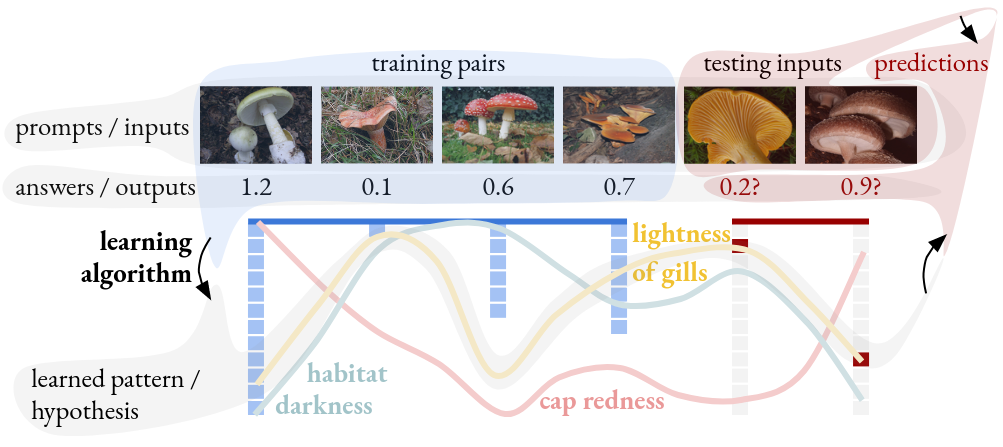
\includegraphics[width=\textwidth]{figures/supervised}\\
          \caption{%
            A program that learns to predict mushrooms' poison levels:
            %
            first takes a list of labeled mushrooms as input (blue blob);
            searches
            through candidate patterns (here, the wiggly curves labeled
            \texttt{lightness of gills}, \texttt{habitat darkness}, and
            \texttt{cap redness}); and returns the pattern that best fits the
            examples.
            %
            Evaluating this pattern on new mushrooms, we predict their poison
            levels (red blob). 
            %
            \par The three bold black arrows show the flow of data from
            training examples to a learned pattern; and from that pattern
            together with testing prompts to predictions.  
            %
            Part of specifying the learning program is specifying the set of candidate patterns to consider.
          }
          \vspace{-0.5cm}
        \end{figure}

        To save ink, say that $\xX$ is the set of possible prompts; $\yY$, of
        possible answers.\bcirc\marginnote{%
          \blarr If we like, we can now summarize the data flow in symbols.  A
          pattern is a function of type $\xX\to\yY$.  And we can model the
          examples from which our program learns as a list of type $(\xX\times
          \yY)^N$.  Then a program that learns from examples has type:
          $$
            \lL : (\xX\times \yY)^N \to (\xX\to \yY)
          $$
          Once we allow uncertainty by letting patterns map to \emph{probability
          distributions} over answers, the type will change to:
          $$
            \lL : (\xX\times \yY)^N \to (\xX\to \text{DistributionsOn}(\yY))
          $$
        }
        In the mushrooms example, $\xX$ contains all
        conceivable mushrooms and $\yY$ contains all conceivable poison
        levels (perhaps all the non-negative real numbers).

      \samsubsubsection{supervised learning}
        We'll soon allow uncertainty by letting patterns map to \emph{probability
        distributions} over answers.
        %
        Even if the prompt is always the same --- say, ``produce a beautiful
        melody'', we may seek to understand the complicated distribution over
        answers.  We might regard our program a success if it can
        generate a variety of good answers.
        %
        So-called \textbf{unsupervised learning} focuses in that way on output
        structure.  By contrast, \textbf{supervised learning} (our subject in
        Unit 1), focuses on the input-output relation; it's interesting when
        the space of prompts is large.\footprint
        %

    \newpage
    \samsubsection{a tiny example: handwritten digit classification}
      \samsubsubsection{meeting the data}
        $\xX = \{\text{grayscale~}28\!\times\!28\text{-pixel images}\}$;
        $\yY=\{{\cya{1}},{\red{9}}\}$.  Each datum $(x,y)$ arises as follows:
        we randomly choose a digit $y\in \yY$, ask a human to write that digit
        in pen, and then photograph their writing to produce $x\in\xX$.\footprint
        %
        \vspace{-0.25cm}
        \begin{figure}
            \centering
          \begin{tabular}{c}
\includegraphics[width=0.75cm]{example-mnist/mnist-trn-00}\\$\red{9}$\\
\includegraphics[width=0.75cm]{example-mnist/mnist-trn-10}\\$\cya{1}$\end{tabular}%
          \begin{tabular}{c}
\includegraphics[width=0.75cm]{example-mnist/mnist-trn-01}\\$\cya{1}$\\
\includegraphics[width=0.75cm]{example-mnist/mnist-trn-11}\\$\red{9}$\end{tabular}%
          \begin{tabular}{c}
\includegraphics[width=0.75cm]{example-mnist/mnist-trn-02}\\$\red{9}$\\
\includegraphics[width=0.75cm]{example-mnist/mnist-trn-12}\\$\cya{1}$\end{tabular}%
          \begin{tabular}{c}
\includegraphics[width=0.75cm]{example-mnist/mnist-trn-03}\\$\red{9}$\\
\includegraphics[width=0.75cm]{example-mnist/mnist-trn-13}\\$\cya{1}$\end{tabular}%
          \begin{tabular}{c}
\includegraphics[width=0.75cm]{example-mnist/mnist-trn-04}\\$\cya{1}$\\
\includegraphics[width=0.75cm]{example-mnist/mnist-trn-14}\\$\red{9}$\end{tabular}%
          \begin{tabular}{c}
\includegraphics[width=0.75cm]{example-mnist/mnist-trn-05}\\$\red{9}$\\
\includegraphics[width=0.75cm]{example-mnist/mnist-trn-15}\\$\red{9}$\end{tabular}%
          \begin{tabular}{c}
\includegraphics[width=0.75cm]{example-mnist/mnist-trn-06}\\$\red{9}$\\
\includegraphics[width=0.75cm]{example-mnist/mnist-trn-16}\\$\red{9}$\end{tabular}%
          \begin{tabular}{c}
\includegraphics[width=0.75cm]{example-mnist/mnist-trn-07}\\$\red{9}$\\
\includegraphics[width=0.75cm]{example-mnist/mnist-trn-17}\\$\cya{1}$\end{tabular}%
          \begin{tabular}{c}
\includegraphics[width=0.75cm]{example-mnist/mnist-trn-08}\\$\cya{1}$\\
\includegraphics[width=0.75cm]{example-mnist/mnist-trn-18}\\$\red{9}$\end{tabular}%
          \begin{tabular}{c}
\includegraphics[width=0.75cm]{example-mnist/mnist-trn-09}\\$\red{9}$\\
\includegraphics[width=0.75cm]{example-mnist/mnist-trn-19}\\$\cya{1}$\end{tabular}%
          \caption{
            Twenty example pairs.  Each photo $x$ is a $28\times 28$ grid of
            numbers representing pixel intensities.  The light gray background
            has intensity $0.0$; the blackest pixels, intensity $1.0$.  Below
            each photo $x$ we display the corresponding label $y$:
            either $y= {\cya{1}}$ or
            $y={\red{9}}$.
            %
            We'll adhere to this color code throughout this tiny example.
          }
        \end{figure}

        \begin{marginfigure}
          \vspace{-3.5cm}
          
\includegraphics[width=0.47\textwidth]{example-mnist/mnist-trn-00}%\\$\red{9}$
            \hspace{0.03\textwidth}
          
\includegraphics[width=0.47\textwidth]{example-mnist/mnist-trn-01}%\\$\cya{1}$
        \end{marginfigure}
        When we zoom in, we can see each photo's $28\times 28$ grid of pixels.
        On the computer, this data is stored as a $28\times 28$ grid of numbers:
        $0.0$ for bright through $1.0$ for dark.
        Our convention will be to name these $28\times28$ grid locations by the
        number of their row (counting starting from top) and then of their column
        (counting starting from the left).  So location $(0,0)$ is the upper
        left corner pixel; location $(27,0)$ is the lower left corner pixel.
        \par\noindent
        \attn{Exercise:} {Where is location $(0,27)$?  $(14,8)$?  $(14,14)$?}
        \par\noindent
        \attn{Exercise:} {What pixel intensities do these two photos have at these three locations?}

        \footprint
        As part of getting to know the data, it's worth taking a moment to
        think about how we would go about hand-coding a digit classifier.  The
        challenge is to complete the pseudocode
        %
        ``\texttt{if (?)\ then predict y=9 else predict y=1}''.
        %
        Well, ${\red{9}}$s tend to have more ink than than ${\cya{1}}$s ---
        should \texttt{(?)}\ threshold by the photo's darkness?
        %
        Or: ${\cya{1}}$s and ${\red{9}}$s tend to have different widths ---
        should \texttt{(?)}\ threshold by the photo's dark part's width?

        \begin{marginfigure}
          \centering
          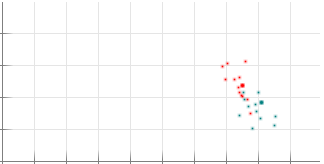
\includegraphics[width=0.99\textwidth]{example-mnist/train-plain}
          \caption{
            Our size-$N=25$ set of training examples, viewed in the
            darkness-width plane.  The vertical \emph{darkness} axis ranges
            $[0.0,0.25]$; the horiziontal \emph{width} axis ranges $[0.0,0.5]$.
            The origin is at the lower left.  Each {\cya{cyan}} dot represents a
            $y={\cya{1}}$ example; each {\red{red}} dot, a $y={\red{9}}$ one.
            %
            The big ${\red{9}}$ above has darkness and width $(0.118, 0.375)$;\
            the big ${\cya{1}}$, $(0.092, 0.404)$.  See where they are in this
            plot?
          }
        \end{marginfigure}

        To make this precise, let's define a photo's \emph{darkness} as its
        average pixel darkness; its \emph{width} as the standard deviation of
        the column index of its dark pixels.  For convenience let's normalize
        both width and darkness to have max possible value $1.0$.  Such
        functions from inputs in $\xX$ to numbers are called
        \textbf{features}.\footprint

        \begin{lstlisting}[language=Python, basicstyle=\footnotesize\ttfamily]
          SIDE = 28
          def darkness(x):
            return np.mean(np.mean(x))
          def width(x):
            return np.std([col for col in range(SIDE)
                               for row in range(SIDE)
                               if 0.5 < x[row][col]  ])/(SIDE/2.0) 
        \end{lstlisting}

        So we can threshold by darkness or by width.  But this isn't very
        satisfying, since sometimes there are especially dark ${\cya{1}}$s or
        wide ${\red{9}}$s. 
        %
        We thus arrive at the idea of using \emph{both} features: ${\red{9}}$s
        are darker than ${\cya{1}}$s \emph{even relative to their
        width}.  So we might write something like
        \texttt{2*darkness(x)-width(x)>0} for\bcirc\marginnote{%
          \blarr That factor of
          $2$ comes from our observation that darkness and tends to be $0.15$
          while width tends to be around $0.30$.
        } our condition.

        \begin{lstlisting}[language=Python, basicstyle=\footnotesize\ttfamily]
          def hand_coded_predict(x):
            return 9 if 2*darkness(x)-width(x)>0 else 1
        \end{lstlisting}

        \noindent
        \attn{Exercise:} {Beyond width and darkness, what features do you think
        might help us to separate digits $1$ from $9$?
        How about $0$ from $9$?}\footprint

    \newpage
      \samsubsubsection{candidate patterns}
        We can generalize the hand-coded hypothesis from the previous passage
        to other coefficients besides $1\cdot \text{width}(x) -
        2\cdot\text{darkness}(x)$.  We let our set $\hH$ of candidate patterns
        contain all ``linear hypotheses'' $f_{a,b}$ defined by:\footprint
        $$
          f_{a,b}(x) = {\red{9}} \text{~~if~~} a\cdot\text{darkness}(x) + b\cdot\text{width}(x) > 0 \text{~~else~~} {\cya{1}}
        $$ 
        Each $f_{a,b}$ makes predictions of $y$s given $x$s.  As we change $a$
        and $b$, we get different predictors, some more accurate than others.

        \begin{lstlisting}[language=Python, basicstyle=\footnotesize\ttfamily]
          def predict(x,a,b):
            return 9 if a*width(x) + b*darkness(x) > 0 else 1
        \end{lstlisting}

        \noindent
        \attn{Exercise:} {how do $\offourline{0}$'s $3$ straight lines and
        $\offourline{1}$'s $3$ marked points correspond?}\footprint

      \samsubsubsection{optimization}
        Let's write a program $\lL$ that given a list of \emph{training
        examples} produces a hypothesis in $h \in \hH$ that helps us predict
        the labels $y$ of yet-unseen photos $x$ (\emph{testing examples}).
        Insofar as training data is representative of testing data, it's
        sensible to return a $h\in \hH$ that correctly classifies maximally
        many training examples.\footprint
        %
        To do this, let's make $\lL$ loop over all integer pairs $(a,b)$ in
        $[-99,+99]$:  %to minimize the number of misclassified training examples. 
        \begin{lstlisting}[language=Python, basicstyle=\footnotesize\ttfamily]
          def accuracy_on(examples,a,b):
            return sum(1.0 for x,y in examples if predict(x,a,b)==y)/len(examples)

          def best_hypothesis():
            return max((accuracy_on(training_data, a, b), (a,b))
                       for a in range(-99,100) 
                       for b in range(-99,100))
        \end{lstlisting}

        \begin{figure}[h]
            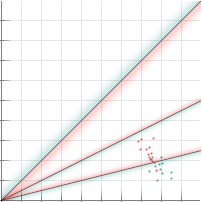
\includegraphics[width=0.24\textwidth]{example-mnist/train.png}%
            \hspace{0.005\textwidth}%
            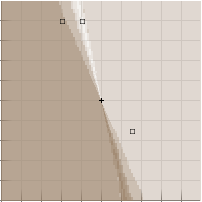
\includegraphics[width=0.24\textwidth]{example-mnist/train-scat.png}%
            \hspace{0.02\textwidth}%
            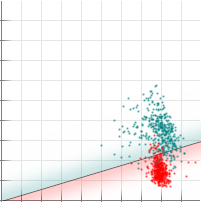
\includegraphics[width=0.24\textwidth]{example-mnist/test.png}%
            \hspace{0.005\textwidth}%
            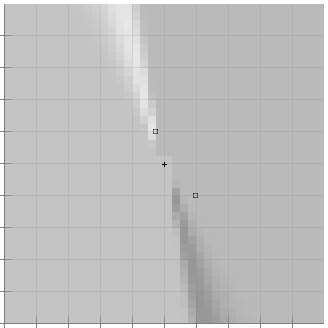
\includegraphics[width=0.24\textwidth]{example-mnist/test-scat.png}
            %
            \caption{
              \textbf{Training
              ($\protect\offourline{01}$) and testing
              ($\protect\offourline{23}$).}
              %
              $3$ hypotheses classify
              training data in the darkness-width plane ($\protect\offourline{0}$).
              %
              Each point in the $(a,b)$ plane ($\protect\offourline{1}$) represents
              a hypothesis; we shade them by the fraction of training
              data they misclassify: darker means less accurate.
              %
              Panes $\protect\offourline{23}$ show the same for
              \emph{testing} data.
              %
              $\protect\offourline{02}$'s axes range $[0, 0.5]$.
              $\protect\offourline{13}$'s axes range $[-99,+99]$. 
            }
        \end{figure}


        When we feed $N=25$ training examples to $\lL$, it produces
        $(a,b)=(80,-20)$ as a minimizer of \textbf{training error}, i.e.,
        of the fraction of training examples misclassified.  It misclassifies
        only $12\%$ of training examples.\footprint Yet the same
        hypothesis misclassified a greater fraction --- $18\%$ --- of fresh,
        yet-unseen testing examples.
        %
        That latter number --- called the \textbf{testing error} --- represents
        our program's accuracy ``in the wild'';
        it's the number we most care about.  The difference between training
        and testing error is the difference between our score on a practice
        exam or homework, where we're allowed to review mistakes we made and
        do a second try, versus our score on an exam, where we don't know the
        questions beforehand and aren't allowed to change our answers once we
        get our grades back.

        \noindent
        \attn{Exercise:} {visualize $f_{a,b}$'s error on $N=1$ example as a 
        function of $(a,b)$.}\footprint

      \samsubsubsection{error analysis}
        Intuitively, our testing error of $18\%$ comes from three sources:
        \textbf{(a)} the failure of our training set to be representative of our testing set; 
        \textbf{(b)} the failure of our program to exactly minimize training error over $\hH$;
        \textbf{(c)} and the failure of our hypothesis set $\hH$ to contain ``the true'' pattern. 

        These errors are respectively called
        \textbf{generalization error},
        \textbf{optimization   error},
        \textbf{approximation  error}.

        Here, we got optimization error $\approx 0\%$ (albeit by
        \emph{unscalable brute-force}).  Because optimization error is zero in
        our case, the approximation error and training error are the same:
        $\approx12\%$.  The approximation error is so high because our straight
        lines are \emph{too simple}: width and darkness lose useful
        information, and the ``true'' boundary between training digits looks
        curved.\footprint
        %
        Finally, our testing error $\approx 18\%$ exceeds our training error.
        We thus suffer a generalization error of $\approx 6\%$: we \emph{didn't
        perfectly extrapolate} from training to testing situations.
        %
        In 6.86x we'll address all three italicized issues.

        \noindent
        \attn{Exercise:} {why is generalization error usually positive?}\footprint



        %\newpage
    \samsubsection{supervised learning framework}
      \samsubsubsection{formalism}
        Draw training examples $\sS : (\xX\times \yY)^N$ %a list of examples
        from nature's distribution $\dD$ on $\xX\times \yY$.  A pattern
        $f:\xX\to \yY$ has \textbf{training error}
        $
           \Ein(f) = \Pp_{(x,y)\sim \red{\sS}}[f(x)\neq y] 
        $, an average over examples; and \textbf{testing error}
        $
           \Eout(f) = \Pp_{(x,y)\sim \red{\dD}}[f(x)\neq y] 
        $, an average over nature.  A \emph{learning program} is a function 
        $
            \lL : (\xX\times \yY)^N \to (\xX\to \yY)
        $; we want to design $\lL$ so that it maps typical $\sS$s to $f$s with
        low $\Eout(f)$.\marginnote{%
          %  TODO: mention extereme class-imbalance and bayesian *decision* theory 
        }

      \samsubsubsection{learning error}
        As in the previous subsection's tiny example,  
        we often define
        $\lL$ to roughly
        minimize $\Ein$ over a
        set $\hH \subseteq (\xX\to \yY)$ of candidate patterns.  Then $\Eout$
        decomposes
        into the failures
        of
        $\Ein$ to estimate $\Eout$ (generalization),
        of
        $\lL$ to minimize $\Ein$ (optimization), and 
        of
        $\hH$ to contain
        nature's
        truth (approximation): 
        \newcommand{\minf}[1]{{\inf}_{\hH}}
        \begin{align*}
            \Eout(\lL(\sS)) 
            =~&\Eout(\lL(\sS))      &-\,\,\,&      \Ein(\lL(\sS)) &~\}~& \text{\textbf{generalization} error} \\
            +~&\Ein(\lL(\sS))       &-\,\,\,& \minf{\hH}(\Ein(f)) &~\}~& \text{\textbf{optimization} error} \\
            +~&\minf{\hH}(\Ein(f))  &       &                     &~\}~& \text{\textbf{approximation} error}  
        \end{align*}
        These terms are in tension.  For example, as $\hH$ grows, the
        approx.\ error may decrease while the gen.\ error may
        increase --- this is the ``\textbf{bias-variance} tradeoff''.

      \samsubsubsection{workflow}
      %\samsubsubsection{workflow: framing}
        \emph{Framing} is about knowing our data and knowing what problem we
        want it to help solve.  Framing includes \emph{factorizing} a complex
        prediction problem into simple classification and regression problems;
        preparing and \emph{splitting} the consequent example pairs into
        training, development, and testing sets, and and \emph{visualizing} the
        training data to weigh our intuitions. 

      %\samsubsubsection{workflow: modeling}
        \emph{Modeling} is about presenting our data in a way that is easy to
        digest for the computer --- in a way that easily found patterns are
        intuitively likely to be accurate. 
        %
        This is the key stage where we will inject our \emph{domain knowledge}
        --- that is, our human experience and intuition about which factors
        are likely to help with prediction.
        %
        Modeling includes \emph{featurizing} our inputs and \emph{regularizing}

        by choosing a class of \emph{priors} and symmetries.

      %\samsubsubsection{workflow: training}
        \emph{Training} is about getting the computer to digest the data we've
        given it.  Under the hood, the computer will try a zillion candidate
        patterns until it hits upon one that explains the examples relatively
        well.  Above, we used brute force search; soon we'll learn more
        efficient approximate algorithms such as \emph{gradient descent}. 
        Training also involves \emph{model selection}: selecting from several
        qualitatively different models one that best predicts the development
        set.

      %\samsubsubsection{workflow: harvesting}
        \emph{Harvesting} is about doing stuff with the pattern the computer
        settled on after it tried a zillion candidates.  We can derive insights
        from the pattern itself (which factors ended up being most important?)
        and we can predict outputs corresponding to fresh inputs.
        %
        Qualifying both applications is the pattern's quality.  To assess this,
        we measure its accuracy on our held-out testing data.


        \newpage
  \samsection{appendix: python programming}

    \samsubsection{python setup}
      \samquote{
        Displace one note and there would be diminishment, displace one phrase
        and the structure would fall.
      }{antonio salieri, on wolfgang mozart's music, as untruthfully portrayed in \emph{Amadeus}}

      \samsubsubsection{what's python?}
        Python is a popular programming language.  Its heart is the
        \textbf{Python interpreter}, a computer program that takes a plain old
        text file such as this two-liner\bcirc\marginnote{%
          \blarr The instruction \texttt{print} just displays some text
          onto our screen.  For example, the first line of this program 
          displays \texttt{hello, world!} onto our screen.  This instruction
          doesn't rely on or activate any ink-on-paper printing machines.
        } ---
        \begin{lstlisting}[language=Python, basicstyle=\footnotesize\ttfamily]
          print('hello, world!')
          print('cows and dogs are fluffy')
        \end{lstlisting}
        --- and executes the instructions contained in that text file.  The
        jargon is that these textual instructions are \textbf{source code}.

        The instructions have to be in a certain, extremely rigid format in
        order for the interpreter to understand and execute them.  That's why
        they call Python a \emph{language}: it has its own rigid grammar
        and its own limited vocabulary.  If the
        interpreter encounters incorrectly formatted instructions --- if even a
        single punctuation mark is missing or a --- the interpreter will display a
        bit of text in addition to the word \texttt{Error} and immediately
        after abort its mission.\bcirc\marginnote{%
          \blarr Adventure boldly when learning Python!  It might feel
          catastrophic when you encounter an error and the interpreter
          `dies'.  But (unless you go out of your way to use special
          instructions we won't teach in class) these errors won't hurt your
          computer.  There aren't any lasting effects. 
          %
          So \textbf{errors are hints, not penalties}. 
          If you encounter an
          error, just modify your instructions to address that error, then run
          the interpreter again.
          %
          Engage in a fast feedback cycle (\emph{I'll try this... error...
          okay how about this...  different error... hmm let's think...}) 
          to learn to program well.
        }

        We'll use Python in 6.86x to instruct our computer to analyze and learn
        from data.  The gigantic project of instructing a computer to learn is
        a bit like teaching a person by mail.  We never see them: we only
        exchange words back and forth.  They have never seen a horse, and yet
        we want to teach them to distinguish horses from zebras from donkeys
        from tapirs from rhinos.  Though severely limited in their vocabulary
        and their ability to appreciate analogies and similarities, they are
        extraordinarily meticulous, patient, and efficient. 
        %
        That's what programming will be like.

        At this point, you might have several questions:
        \begin{description}
          \item[\textbf{Picking up the pen:}] How do I install and use the Python
               interpreter? 
          \item[\textbf{Writing sentences:}] What syntax rules must my
               instructions obey in order for the interpreter to understand
                that I want it do such-and-such task? 
          \item[\textbf{Composing essays:}] How do I organize large programs?
          \item[\textbf{Teaching via mail:}] What instructions make
               make the computer learn from data?
        \end{description}
        This subsection and the next three subsections address these four
        questions in turn.

      \samsubsubsection{which things we'll set up}
        Let's set up Python by installing the Python interpreter.
        %
        Actually, I should say \emph{a} Python interpreter: each of the many
        software tools we'll use in 6.86x has a zillion versions; it can get
        confusing tracking which versions coexist and which clash.  We will use
        \textbf{Python version 3.8} throughout 6.86x.

        Beyond the Python interpreter, there is an ecosystem of useful tools:
        machine learning modules that help us avoid reinventing the wheel; a
        rainbow of feature-rich text editors specialized for writing Python code;
        and a package manager called \texttt{conda} that eases the logistics
        nightmare of coordinating the versions we have of each tool.

      \samsubsubsection{setup on windows}
        %If you're on
        %Windows 10 or higher, then similar steps should work after you set up
        %the ``Linux Subsystem for Windows.''
      \samsubsubsection{setup on macOS}
      \samsubsubsection{setup on linux}
        I'll assume we're working with Ubuntu 20 or
        related.  If you're on a different Linux, then similar
        steps should work --- google search to figure out how.  

        \attnsam{FILL IN: how to run, comments, basic stdIO}
        \attnsam{line by line HELLO WORLD; string type}
        \attnsam{line by line FAHRENHEIT KELVIN CELSIUS; float and integer types}

    \newpage
    \samsubsection{python basics}
      % use-mention distinction; syntax-semantic.s  Asimov ROBOT????
      % TODO: figure out what I meant by the comment line directly above
      \samquote{
        If I have not seen as far as others, it is because giants were standing
        on my shoulders.
      }{hal abelson}
      \marginnote{%
        Once you learn how to program, I highly recommend reading Edsger
        Dijkstra's \emph{A Discipline of Programming}.  That book contains many
        beautiful viewpoints that made me a better programmer.
      }

      \samsubsubsection{output and sequencing}
        Try this one-liner:
        \begin{lstlisting}[language=Python, basicstyle=\footnotesize\ttfamily]
          print('hello!')
        \end{lstlisting}
        Now try this:
        \begin{lstlisting}[language=Python, basicstyle=\footnotesize\ttfamily]
          print(686)
        \end{lstlisting}
        We execute multiple instructions in sequence by placing them on
        successive lines:
        \begin{lstlisting}[language=Python, basicstyle=\footnotesize\ttfamily]
          print('hello!')
          print(6)
          print(86)
          print('goodbye!')
        \end{lstlisting}

      \samsubsubsection{state and assignment}
        Try this two-liner:
        \begin{lstlisting}[language=Python, basicstyle=\footnotesize\ttfamily]
          x = 686
          print(x)
        \end{lstlisting}
        And this three-liner:
        \begin{lstlisting}[language=Python, basicstyle=\footnotesize\ttfamily]
          x = 686
          x = 123
          print(x)
        \end{lstlisting}
        Does the following print the same thing?
        \begin{lstlisting}[language=Python, basicstyle=\footnotesize\ttfamily]
          x = 123
          x = 686
          print(x)
        \end{lstlisting}
        What do you predict this does:
        \begin{lstlisting}[language=Python, basicstyle=\footnotesize\ttfamily]
          x = 123
          print(x)
          x = 686
          print(x)
        \end{lstlisting}
        %
        Above, \texttt{x} names a \textbf{variable}.  A variable stores some
        value at each point in time; it might store different values at
        different times.  We make a variable just by mentioning it in an
        \textbf{assignment} instruction such as \texttt{x=123}.   We get to
        choose each variable's name however we'd like; a variable may have a
        one-letter name or a longer name:\bcirc\marginnote{%
          \blarr Naming rules: the first character must belong to the English
          alphabet (so there are $26$ lower case choices plus $26$ upper case
          choices).  Each subsequent character is either an underscore (that's
          the symbol that looks like \texttt{\_}), a digit (\texttt{0} through \texttt{9}),
          or a member of the English alphabet.
          %
          The following names are forbidden, since they already mean
          something else in Python:
            \texttt{assert},
            \texttt{bool},
            \texttt{break},
            \texttt{chr},
            \texttt{class},
            \texttt{continue},
            \texttt{def},
            \texttt{dict},
            \texttt{elif},
            \texttt{else},
            \texttt{enumerate},
            \texttt{except},
            \texttt{float},
            \texttt{for},
            \texttt{if},
            \texttt{import},
            \texttt{input},
            \texttt{int},
            \texttt{lambda},
            \texttt{len} 
            \texttt{list},
            \texttt{max},
            \texttt{min},
            \texttt{ord},
            \texttt{print},
            \texttt{range},
            \texttt{round},
            \texttt{set},
            \texttt{str},
            \texttt{sum},
            \texttt{try},
            \texttt{type},
            \texttt{while},
            \texttt{with},
            \texttt{zip}.
          %
          For a full list of forbidden names, google search \emph{list of
          Python keywords and built-in functions}.
        }
        \begin{lstlisting}[language=Python, basicstyle=\footnotesize\ttfamily]
          my_favorite_number = 123
          print(my_favorite_number)
          my_favorite_number = 686
          print(my_favorite_number)
        \end{lstlisting}
        %
        We can use multiple \textbf{variables}:
        \begin{lstlisting}[language=Python, basicstyle=\footnotesize\ttfamily]
          x = 123
          y = 686
          print(x)
        \end{lstlisting}
        What do you think the following prints?
        \begin{lstlisting}[language=Python, basicstyle=\footnotesize\ttfamily]
          x = 123
          y = 686
          x = y
          print(x)
          print(y)
        \end{lstlisting}

      \samsubsubsection{arithmetic}
        We can put math on the right hand side of assignments:\marginnote{%
          \attnsam{variable cube; assignment as shearing}
        }
        \begin{lstlisting}[language=Python, basicstyle=\footnotesize\ttfamily]
          x = 123
          y = x*2 + 1000
          print(x)
          print(y)
        \end{lstlisting}
        What do you think the following prints?
        \begin{lstlisting}[language=Python, basicstyle=\footnotesize\ttfamily]
          x = 123
          x = x*2 + 1000
          print(x)
        \end{lstlisting}
        %
        What do you think the following prints?
        \begin{lstlisting}[language=Python, basicstyle=\footnotesize\ttfamily]
          x = 123
          x = x*2 + 1000
          print(x)
        \end{lstlisting}
        %
        Here's a more involved example.  See what it's trying to do?
        \begin{lstlisting}[language=Python, basicstyle=\footnotesize\ttfamily]
          target = 20.0
          x = 4.0
          x = x - 0.01*(x*x*(x - target/x)) 
          x = x - 0.01*(x*x*(x - target/x)) 
          x = x - 0.01*(x*x*(x - target/x)) 
          x = x - 0.01*(x*x*(x - target/x)) 
          x = x - 0.01*(x*x*(x - target/x)) 
          x = x - 0.01*(x*x*(x - target/x)) 
          y = x*x
          message = str(x) + ' squares to ' + str(y) + ' which nearly equals ' + str(target) 
          print(message)
        \end{lstlisting}
        If you successfully executed the above code, then you have officially
        done \textbf{iterative optimization}!  Notice the repeated instruction
        \texttt{x=(target/x+x)/2}.  Each time this instruction is executed,
        \texttt{x}'s value gets closer to the square root of \texttt{target}'s
        value.  6.86x features this theme of ``repeatedly improve in order to
        optimize'' in the guises of \textbf{gradient descent} and of
        \textbf{expectation maximization}.  In fact, the code above is gradient
        descent on the loss function $\ell(x) = (x^2-\text{target})^2$.


      \samsubsubsection{ints, floats, strings, bools}
        %We speak of a variable having a value.
        %A fixed variable may have different values at different times.
        The variable values we work with might be numbers,
        or pieces of text, or answers to a true-false question, or
        something else.  The kind of thing a value is is called that value's
        \textbf{type}.
        %
        We use the jargon \textbf{string} or \textbf{str}
        for the type of thing that chunks of text are.  For example, much as
        \texttt{3.141} is a number, \texttt{'hello, world!'} is a string.
        %
        The jargon \textbf{bool} denotes the type of thing that can answer
        a true-or-false question.  For example, while the value \texttt{'True'}
        is a string, the value \texttt{True} is a bool.  So is \texttt{False}.
        Those are the only two possible bools.
        %
        We'll distinguish two kinds of numeric value: values who by dint of
        their type are integers, and values that might or might not be
        integers.  The jargon word for the former's type is \textbf{int};
        for the latter's, \textbf{float}.\bcirc\marginnote{%
           \blarr Historically, \textbf{int} abbreviates \emph{integer} and
           \textbf{float} stands for \emph{floating decimal point} (except with
           binary instead of decimal).  The poetic image is of a decimal point
           that can drift around as if in a sea:
           \texttt{31.41}, \texttt{3.141}, \texttt{0.3141},
           \texttt{0.03141}, etc.
           %
           Floats thus stand in contrast to ``banker's'' numbers, which do not
           track differences smaller than one-hundredth of a dollar.
           %
           %Floats can express very large and very small quantities such as
           %\texttt{314100000000} and \texttt{0.000000000003141}.
        }  For example, when we write \texttt{5} or \texttt{686}, the
        interpreter understands those values to be ints; when we write
        \texttt{5.0} or \texttt{0.003141}, the interpreter understands those
        values to be floats.

        Different types support different operations and activities.  For
        example, it makes sense to multiply two floats but not two strings.
        And if \texttt{x} is a variable containing a value of type
        \texttt{int}, then it makes sense to access a string's \texttt{x}th
        character.  But that wouldn't make sense with \texttt{int} replaced by
        \texttt{float}.

        Here's a flash summary of several common operations: 

        \begin{table}[h]
          \begin{tabular}{cccc}
            \textsc{operation}  &\textsc{input type(s)}           &\textsc{output type} &\textsc{how to write it}               \\
            \hline
            add                 &\texttt{int}   , \texttt{int}    &\texttt{int}         &\texttt{x+y}                           \\
            add                 &\texttt{int}   , \texttt{float}  &\texttt{float}       &\texttt{x+y}                           \\
            add                 &\texttt{float} , \texttt{int}    &\texttt{float}       &\texttt{x+y}                           \\
            add                 &\texttt{float} , \texttt{float}  &\texttt{float}       &\texttt{x+y}                           \\
            literal int 5       &                                 &\texttt{int}         &\texttt{5}                             \\
            literal float 5.0   &                                 &\texttt{float}       &\texttt{5.0}                           \\
            \hline
            count characters    &\texttt{str}                     &\texttt{int}         &\texttt{len(s)}                        \\
            $n$th character     &\texttt{str}   , \texttt{int}    &\texttt{str}         &\texttt{s[n]}                          \\
            concatenate         &\texttt{str}   , \texttt{str}    &\texttt{str}         &\texttt{left\_str+right\_str}          \\
            literal string '5'  &                                 &\texttt{str}         &\texttt{'5'}                           \\
            \hline
            round toward zero   &\texttt{float}                   &\texttt{int}         &\texttt{int(f)}                        \\
            promote to float    &\texttt{int}                     &\texttt{float}       &\texttt{float(n)}                      \\
            render              &\texttt{int}                     &\texttt{str}         &\texttt{str(n)}                        \\
            render              &\texttt{float}                   &\texttt{str}         &\texttt{str(f)}                        \\
            parse               &\texttt{str}                     &\texttt{int}         &\texttt{int(s)}                        \\
            parse               &\texttt{str}                     &\texttt{float}       &\texttt{float(s)}                      \\
            \hline
            negation            &\texttt{bool}                    &\texttt{bool}        &\texttt{not x}                         \\
            conjunction         &\texttt{bool}  , \texttt{bool}   &\texttt{bool}        &\texttt{x and y}                       \\
            disjunction         &\texttt{bool}  , \texttt{bool}   &\texttt{bool}        &\texttt{x or y}                        \\
            literal bool False  &                                 &\texttt{bool}        &\texttt{False}                         \\
            \hline
            check equality      &\texttt{str}   , \texttt{str}    &\texttt{bool}        &\texttt{x==y}                          \\
            check equality      &\texttt{int}   , \texttt{int}    &\texttt{bool}        &\texttt{x==y}                          \\
            check at-most       &\texttt{int}   , \texttt{int}    &\texttt{bool}        &\texttt{x<=y}                          \\
            check at-least      &\texttt{int}   , \texttt{int}    &\texttt{bool}        &\texttt{x>=y}                          \\
            check at-most       &\texttt{float} , \texttt{float}  &\texttt{bool}        &\texttt{x<=y}                          \\
            check at-least      &\texttt{float} , \texttt{float}  &\texttt{bool}        &\texttt{x>=y}                          \\
          \end{tabular}
          \caption{%
            Python supports all of addition, subtraction,
            multiplication, and exponentiation: we use the symbols
            \texttt{+}, \texttt{-}, \texttt{*}, \texttt{/}, and \texttt{**}.
            For brevity we listed only addition in this table.
          }
        \end{table}

        That's a lot to take in.  Let's digest by seeing these operations
        in action:
        \begin{lstlisting}[language=Python, basicstyle=\footnotesize\ttfamily]
          my_string = 'dear world,' 
          my_string = my_string + ' my favorite number is ' + str(389)
          print(my_string)
        \end{lstlisting}
        And
        \begin{lstlisting}[language=Python, basicstyle=\footnotesize\ttfamily]
          s = 'hi, world!' 
          my_message = 'my string s has ' + str(len(my_string)) + 'many characters,'
          my_message = my_message + ' of which the first and last couple are:'
          my_message = my_message + s[0] + s[1] + '...' + s[8] + s[9]
          print(my_message)
        \end{lstlisting}
        And
        \begin{lstlisting}[language=Python, basicstyle=\footnotesize\ttfamily]
          x = 3 * 5.01
          y = 3.01 * 5
          s = 'abcdefghijklmnopqrstuvwxyz'
          is_nearly_equal = (y-0.1 < x) and (x < y+0.1) 
          print(is_nearly_equal)
        \end{lstlisting}

        \newpage
      \samsubsubsection{input}
      \samsubsubsection{conditionals}% also mention trivalent CHOICE operator?
      \samsubsubsection{iteration}

        %
        \marginnote{%
          % for-range idiom; break, continue, else in loops 
        }
      \samsubsubsection{nesting, scope, indentation}
        \attnsam{skip, abort}

      \samsubsubsection{remarks on `types'}
      \samsubsubsection{data in aggregate}%container structures}
        \attnsam{lists, strings, numpy arrays} % no tuples
        \attnsam{dictionaries} % no sets; mention cacheing (and hence also global scope??)
        \attnsam{comprehensions}
        \attnsam{functional idioms}

      \samsubsubsection{example: the restaurant bill}
        Let's write a program that takes a list of prices as command line input
        and displays a grand total including with $6\%$ tax and a variety of
        tips: $9\%,12\%,15\%,18\%,21\%$.  We'll write the program in two
        styles.  Here is a more conceptual style: 
        \begin{lstlisting}[language=Python, basicstyle=\footnotesize\ttfamily]
          import sys
          prices = [float(arg) for arg in sys.argv[1:]] 
          total = sum(prices) 

          with_tax = total * (1.0 + 0.06)
          print('raw price:', total   , 'dollars')
          print('with tax:' , with_tax, 'dollars')
          for tip in range(9, 24, 3):
            with_tax_and_tip = total * (1.0 + 0.06 + tip/100.0) 
            print('tip =', tip, 'percent', '-->', with_tax_and_tip, 'dollars')
        \end{lstlisting}
        We can say the same thing more explicitly as follows: 
        \begin{lstlisting}[language=Python, basicstyle=\footnotesize\ttfamily]
          import sys
          prices = []
          for arg in sys.argv[1:]:
            prices.append(float(arg))
          total = 0.0
          for price in prices:
            total = total + prices

          print('raw price:', total               , 'dollars')
          print('with tax:' , total * (1.0 + 0.06), 'dollars')
          for tip in range(9, 24, 3):
            print('tip =', tip, 'percent', '-->', total * (1.0 + 0.06 + tip/100.0), 'dollars')
        \end{lstlisting}

      \newpage
      \samsubsubsection{example: equation solver}
        Let's write a program that takes a one-variable math equation as a
        command line argument and displays a solution.  We'll restrict
        ourselves to polynomial equations such as \texttt{xxxxx=xx+xx+1+1} (our
        way of writing $x^5=2x^2+2$).  That is, we'll assume the equation has
        no spaces and consists of only the characters \texttt{x}, \texttt{=},
        \texttt{+}, \texttt{1}, \texttt{0}.  Two more valid equations are
        \texttt{xxx+xx+x+1=0} and \texttt{x=xx}.

        \begin{lstlisting}[language=Python, basicstyle=\footnotesize\ttfamily]
          # step 0: read the equation-to-solve from the command line
          import sys
          import numpy as np
          equation = sys.argv[1]

          # step 1: check whether the equation holds for each x in a large
          #         range with fine spacing; print and exit if for one of these
          #         x's the equation holds to tolerance plus-minus 0.1 
          for x in np.arange(-100.00, +100.01, 0.01): 

            # step 1a: initialize accumulator variables that will eventually
            #          represent the values of the equations's left hand and
            #          right hand sides
            index = 0
            left_hand_side = 0.0
            right_hand_side = 0.0
            term = 1.0

            # step 1b: compute the left hand side's numeric value; 
            #          the left hand side ends the moment we see an equals sign
            while equation[index] != '=':
              if   equation[index] == '0': term = term * 0.0
              elif equation[index] == '1': term = term * 1.0
              elif equation[index] == 'x': term = term * x 
              else:
                left_hand_side = left_hand_side + term
                term = 1.0

            # step 1c: skip the equals sign
            index = index + 1

            # step 1d: compute the right hand side's numeric value;
            #          the right hand side ends when our equation ends 
            while index != len(equation):
              if   equation[index] == '0': term = term * 0.0
              elif equation[index] == '1': term = term * 1.0
              elif equation[index] == 'x': term = term * x 
              else:
                right_hand_side = right_hand_side + term
                term = 1.0

            # step 1e: check whether the left and right hand sides are nearly
            #          equal.  if they are, report and exit 
            difference = left_hand_side-right_hand_sided
            if -0.1<difference and difference<+0.1:
              print('x =', x, 'solves', equation, 'with error only', difference)
              sys.exit()

          # step 2: report that the search for a solution was unsuccessful.
          #         since step 1e exits when a solution is found, the
          #         interpreter will get to step 2 only if no solution is found
          print('no solution found to desired tolerance')
        \end{lstlisting}

    \newpage
    \samsubsection{structuring code}
      %\samquote{
      %}{}

      \samsubsubsection{routines}
        %\attnsam{mention SCOPE somewhere (perhaps earlier than this passage?)}
        %\attnsam{lambdas}
        \attnsam{\texttt{def}d functions (ordinary args, return)}
        \attnsam{interfaces: (kwargs; None as default return value; sentinels; more)}
        \attnsam{code architecture and hygiene}
      \samsubsubsection{more input/output}
        \attnsam{print formatting and flushing}
        \attnsam{basic string manipulations (strip, join, etc)}
        \attnsam{file io}
        \attnsam{command line arguments}
        \attnsam{example: read csv}
        %
        \attnsam{random generation and seeds??}
      \samsubsubsection{how not to invent the wheel} %modules: os, numpy, matplotlib}
        \attnsam{matplotlib.plot}
        \attnsam{numpy}
        \attnsam{os}
        \attnsam{package managers etc}

    \newpage
    \samsubsection{numpy and friends}
      \samsubsubsection{arrays aka tensors}
        \attnsam{}
        \attnsam{}
        \attnsam{}
        \attnsam{}
      \samsubsubsection{images: viewing, representing, rendering}
      \samsubsubsection{gradient descent done manually}
      \samsubsubsection{gradient descent in pytorch}
      \samsubsubsection{gradient descent in tensorflow}

\end{document}

